\chapter{Tree}
\label{cha:tree}

\section{前序中序求后序}

给出一个二叉树的前序遍历 GDAFEMHZ 和中序遍历 ADEFGHMZ, 求后序遍历。
首先,二叉树的前序遍历,中序遍历,后序遍历的区别是根节点是先、中、
后访问。问题的关键是:

\begin{enumerate}
\item 前序遍历的第一个节点是根节点;
\item 在中序遍历里找到根结点,其左边是左子树节点,右边是右子树节点;
\item 对左子树重复上面两步;
\item 对右子树重复上面两步。
\item 二叉树被求出,从而得到对应的后序遍历。
\end{enumerate}

上面的例子里,从前序遍历知 G 是根节点,从后序遍历知,左子树是ADEF,
右子树是 HMZ, 此顺序就是左子树的中序遍历顺序。

\begin{figure}[h]
  \centering
  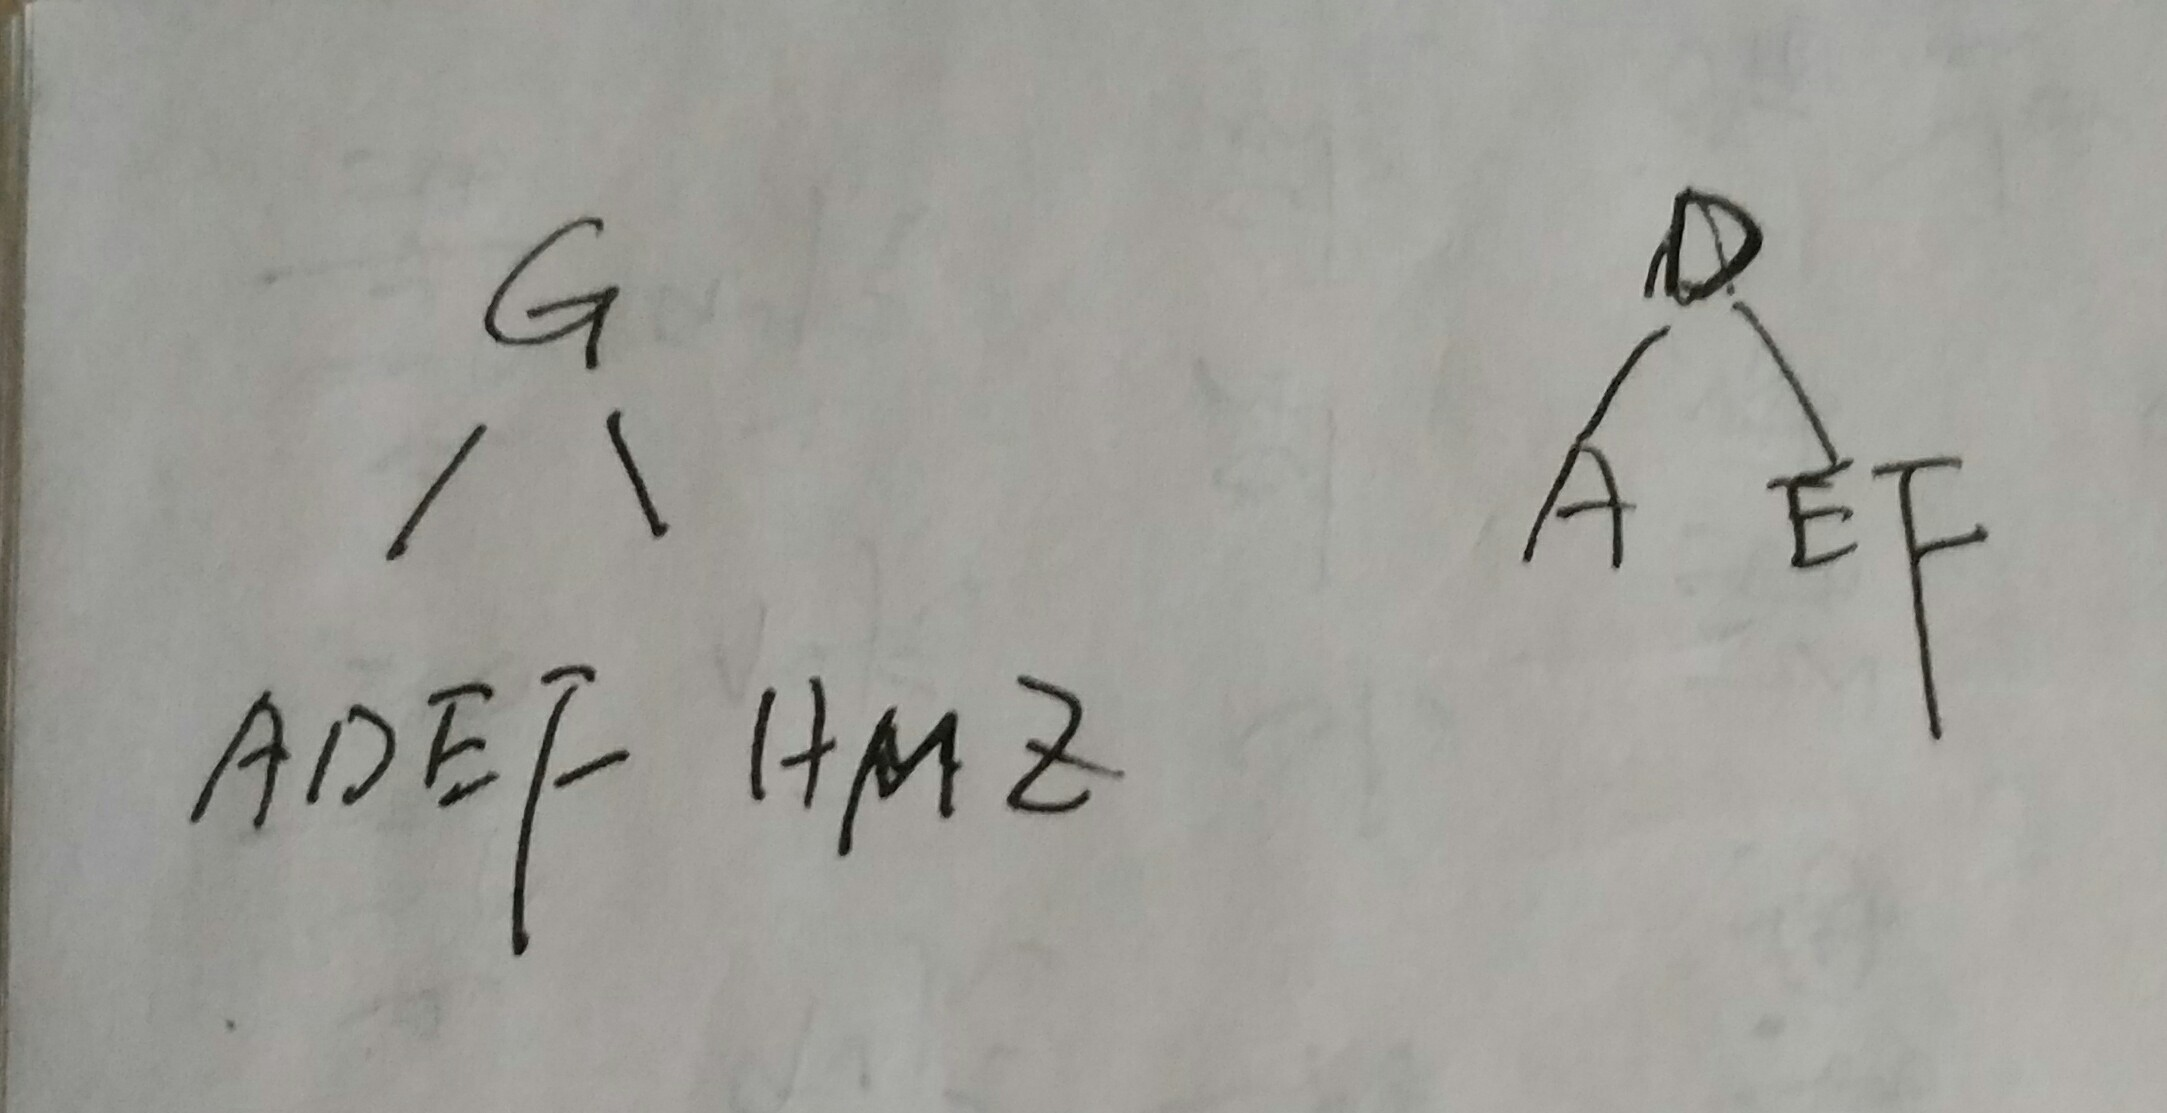
\includegraphics[width=.5\textwidth]{BinaryTreeTraversal}
\end{figure}

但还要找到对应的前序顺序。对左子树 ADEF 来说,在前序遍中的顺序
是 DAFE,说明左子树的根节点是 D, 从其中序顺序可知,左子树是 A, 右子
树是 EF. 重复此过程即可得出二叉树,再得出后序遍历 AEFDHZMG.

同理,已知后序遍历和中序遍历,也可求出前序遍历。唯一的区别是后序遍
历的最后一个节点是根节点,每次找根节点时从最后找。不管是哪种题,中
序遍历一定要有!

%%% Local Variables:
%%% mode: latex
%%% TeX-master: "main"
%%% End:
